\section{Solution Modify existing LaTeX container}
Find existing LaTeX container image
Add missing needed packages
Fix warnings/errors (mktexpk for generating missing fonts)
Integrate/Use container in project.


%\begin{figure}[!h]
%\centering
%\begin{tikzpicture}
%  \node (r1) at (0,0) [draw, align=center, minimum height=2cm,minimum width=2cm] {Pull};
%  \node (r2) at (5,0)  [draw, align=center, minimum height=2cm,minimum width=2cm] {Use};
%  \node (r3) at (10,0) [draw, align=center, minimum height=2cm,minimum width=2cm] {Extend};
%  \node (r4) at (2.5,-5) [draw, align=center, minimum height=2cm,minimum width=2cm] {Build};
%  \node (r5) at (7.5,-5) [draw, align=center, minimum height=2cm,minimum width=2cm] {Push};
%  \draw[arrows={-Latex[length=6pt]}] (r1.east) -- (r2.west);
%  \draw[arrows={-Latex[length=6pt]}] (r2.east) -- (r3.west);
%  \draw[arrows={-Latex[length=6pt]}] (r2.south) -- (r4.north);
%  \draw[arrows={-Latex[length=6pt]}] (r2.south) -- (r5.north);
%\end{tikzpicture}
%\caption{The Development Environment}
%\label{fig:fig1}
%\end{figure}

\usetikzlibrary{calc} 
\usetikzlibrary{shapes}
\begin{figure}[!h]
\centering
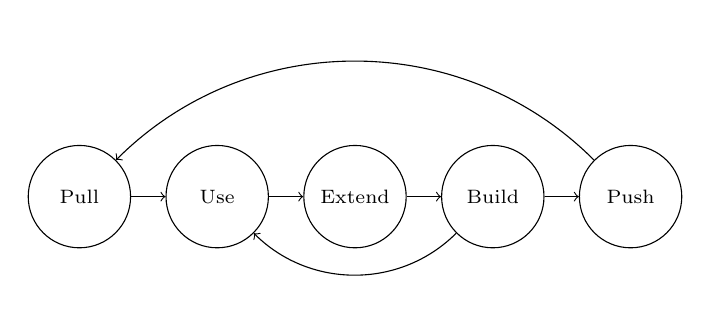
\begin{tikzpicture}
  \node [minimum width=1.3cm,draw,circle] (a) at (0,0) {\scriptsize Pull};
  \node [minimum width=1.3cm,draw,circle] (b) at ($(a)+(1.75,0)$) {\scriptsize Use};
  \node [minimum width=1.3cm,draw,circle] (c) at ($(b)+(1.75,0)$) {\scriptsize Extend};
  \node [minimum width=1.3cm,draw,circle] (d) at ($(c)+(1.75,0)$) {\scriptsize Build};
  \node [minimum width=1.3cm,draw,circle] (e) at ($(d)+(1.75,0)$) {\scriptsize Push};

  \draw[->] (a) -- (b);
  \draw[->] (b) -- (c);
  \draw[->] (c) -- (d);
  \draw[->] (d) -- (e);
  \draw[->] (e) to[out=135,in=45] (a);
  \draw[->] (d) to[out=225,in=315] (b);

\end{tikzpicture}
\caption{Workflow}
\label{fig:fig1}
\end{figure}

%%\lstnewenvironment{code}{%
%%  \lstset{
%%  fillcolor=\color{verbgray},
%%  backgroundcolor=\color{verbgray},
%%  frame=single,
%%  framerule=2pt,
%%  basicstyle=\ttfamily\small,
%%  columns=fullflexible,
%%  lineskip=0pt,  
%%  aboveskip=0pt,
%%  belowskip=0pt }}{}


%%\lstnewenvironment{code}{%
%%  \lstset{
%%  fillcolor=\color{verbgray},
%%  backgroundcolor=\color{verbgray},
%%  basicstyle=\ttfamily\small,
%%  lineskip=0pt,  
%%  aboveskip=0pt,
%%  belowskip=0pt }}{}
%%

\definecolor{shadecolor}{rgb}{.0, .0, .0}

%%\lstset{language=c++,basicstyle=\linespread{1.1}\ttfamily\endnotesize,
%%    xleftmargin=0.0cm, frame=t, framesep=0.15cm, framerule=0pt, tabsize=4,
%%    showspaces=false, showstringspaces=false,showlines=true,
%%    commentstyle=\ttfamily\endnotesize\color{gray},
%%}



\lstnewenvironment{code}
{
 \lstset{
 basicstyle=\ttfamily\scriptsize,
 columns=fullflexible,
 }}{}


\begin{mdframed}[backgroundcolor=black!20,leftmargin=0.0cm,skipabove=0.4cm,hidealllines=true,
  innerleftmargin=0.1cm,innerrightmargin=0.1cm,innertopmargin=0.15cm,innerbottommargin=-0.1cm]

%%\begin{lstlisting}[mathescape, caption = This is some code]

%%\begin{code}[mathescape, caption = This is some code]
\begin{code}
#-----------
# Dockerfile
#-----------
FROM ghcr.io/jmuchovej \
  /devcontainers/latex:2025

USER root

RUN <<EOF
    tlmgr update --self

    tlmgr install \
        pgf booktabs breqn caption \
        ec fc gensymb lastpage \
        makecell mathtools multirow \
        paralist parskip pgf sectsty \
        subfig tex4ht tocbibind 
        
    mktexpk --mfmode / --bdpi 600 \
      --mag 1+0/600 --dpi 600 tcrm1095
    mktexpk --mfmode / --bdpi 600 \
      --mag 1+0/600 --dpi 600 tcrm0900
    mktexpk --mfmode / --bdpi 600 \
      --mag 1+0/600 --dpi 600 tcrm0600
    mktexpk --mfmode / --bdpi 600 \
      --mag 1+0/600 --dpi 600 tcrm0800
EOF

USER vscode
\end{code}
\end{mdframed}






